%%%%%%%%%%%%%%%%%%%%%%%%%%%%%%%%%%%%%%%%%%%%%%%%%%%%%%%%%%%%%%%%%%%%%%%%%%%%%%%%%%
\begin{frame}[fragile]\frametitle{}
\begin{center}
{\Large Introduction to Swift for Tensorflow}
\end{center}
\end{frame}

%%%%%%%%%%%%%%%%%%%%%%%%%%%%%%%%%%%%%%%%%%%%%%%%%%%
\begin{frame}[fragile] \frametitle{Existing Approaches}

Existing approaches for building Neural Networks.

\begin{itemize}
\item Graph building: Pre-specific graph so that it can be made performant at run-time (TensorFlow 1.0) but hard to debug.
\item Eager Execution: Running tensor operations in interpreted code (TensorFlow 2.0), easy to debug, good usability, but bad on performance.
\end{itemize}

Need Usability + Performance.

\end{frame}

%%%%%%%%%%%%%%%%%%%%%%%%%%%%%%%%%%%%%%%%%%%%%%%%%%%
\begin{frame}[fragile] \frametitle{Usability + Performance}

\begin{itemize}
\item Need not just a new library
\item But a new language
\end{itemize}

That's Swift!!.

\end{frame}


%%%%%%%%%%%%%%%%%%%%%%%%%%%%%%%%%%%%%%%%%%%%%%%%%%%%%%%%%%%%%%%%%%%%%%%%%%%%%%%%%%%
\begin{frame}[fragile]\frametitle{Quote}
\begin{lstlisting}
"I always hope that when I start looking at a new language, there will be some mind-opening new ideas to find, and Swift definitely doesn't disappoint. Swift tries to be expressive, flexible, concise, safe, easy to use, and fast. Most languages compromise significantly in at least one of these areas."

- Jeremy Howard
\end{lstlisting}
\end{frame}

%%%%%%%%%%%%%%%%%%%%%%%%%%%%%%%%%%%%%%%%%%%%%%%%%%%%%%%%%%%%%%%%%%%%%%%%%%%%%%%%%%%
\begin{frame}[fragile]\frametitle{Quote}
\begin{lstlisting}
"PyTorch was created to overcome the gaps in Tensorflow. FastAI was built to fill gaps in tooling for PyTorch. But now we're hitting the limits of Python, and Swift has the potential to bridge this gap"

- Jeremy Howard
\end{lstlisting}
\end{frame}


%%%%%%%%%%%%%%%%%%%%%%%%%%%%%%%%%%%%%%%%%%%%%%%%%%%%%%%%%%%%%%%%%%%%%%%%%%%%%%%%%%%
\begin{frame} \frametitle{Swift Ecosystem}
\begin{center}
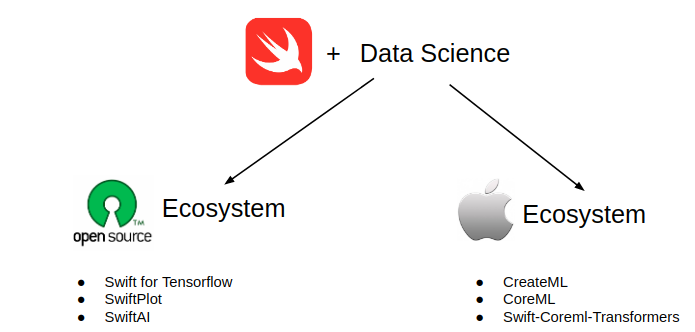
\includegraphics[width=0.9\linewidth,keepaspectratio]{s4tf2}
\end{center}

\begin{itemize}
\item Open-Source Swift runs on any machine.
\item For Apple ecosystem, need Apple machine to work on and you can only build for Apple devices like the iOS, macOS etc.
\end{itemize}

\end{frame}

%%%%%%%%%%%%%%%%%%%%%%%%%%%%%%%%%%%%%%%%%%%%%%%%%%%%%%%%%%%%%%%%%%%%%%%%%%%%%%%%%%%
\begin{frame} \frametitle{iOS/MacOS ML Apps}
\begin{center}
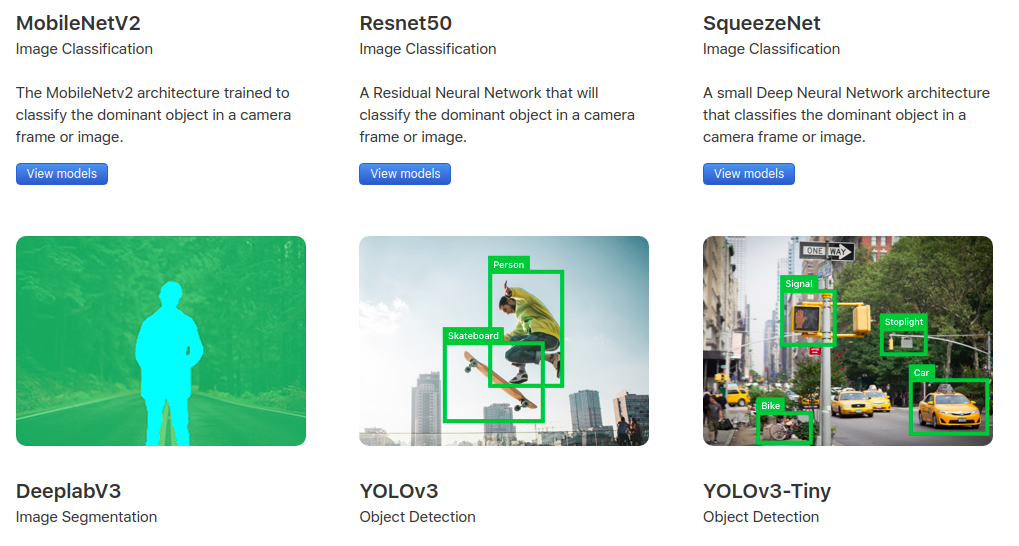
\includegraphics[width=0.9\linewidth,keepaspectratio]{s4tf3}
\end{center}
\end{frame}

%%%%%%%%%%%%%%%%%%%%%%%%%%%%%%%%%%%%%%%%%%%%%%%%%%%
\begin{frame}[fragile] \frametitle{How it all started?}

\begin{itemize}
\item In 2018, started as a small team in Google.
\item Introduced by Chris Lattner at TensorFlow Dev Summit 2018. 
\item On April 27, 2018 Google team has made its first release to public community on their GitHub repository. 
\item Swift is the first mainstream language with first-class language-integrated differentiable programming capabilities
\item But Swift for TensorFlow is still in its infancy stage. Not production ready yet.
\end{itemize}

Still interested? go ahead \ldots

\end{frame}

%%%%%%%%%%%%%%%%%%%%%%%%%%%%%%%%%%%%%%%%%%%%%%%%%%%%%%%%%%%%%%%%%%%%%%%%%%%%%%%%%%
\begin{frame}[fragile]\frametitle{}
\begin{center}
{\Large Why not Python?}
\end{center}
\end{frame}


%%%%%%%%%%%%%%%%%%%%%%%%%%%%%%%%%%%%%%%%%%%%%%%%%%%
\begin{frame}[fragile] \frametitle{Python, Today}

\begin{itemize}
\item Most used language in machine learning
\item Tons of library
\item So, why Swift? What’s wrong with Python?
\end{itemize}

\end{frame}

%%%%%%%%%%%%%%%%%%%%%%%%%%%%%%%%%%%%%%%%%%%%%%%%%%%
\begin{frame}[fragile] \frametitle{Why not Python?}

\begin{itemize}
\item To put it bluntly, Python is slow. 
\item Also, Python is not great for parallelism.
\item Python is usable, but inside its mostly \lstinline|C, C++|
\item External binaries:  limits developers to working on a small portion of the algorithm’s surface area. Cant debug in.
\item Library abstractions: you’ll have to use \lstinline|tf.print| and build a print node and not python \lstinline|print|
\end{itemize}

\end{frame}

%%%%%%%%%%%%%%%%%%%%%%%%%%%%%%%%%%%%%%%%%%%%%%%%%%%
\begin{frame}[fragile] \frametitle{Why Swift?}

\begin{itemize}
\item Swift allows you to program at a very high level, in an almost Pythonic way, while at the same time being really fast.
\item Fast, about 10x than Python.
\item No dynamic type changes. Strict at compile level.
\item Swift makes extensive use of closures (lambda functions),
\item In built differentiation, core to ML.
\item \lstinline|extension|, which allows us to add new functionality to any type, including the basic types.
\item Python interoperability
\item Finally, when you want to run production code, you can compile it and take advantage of the great optimization LLVM provides
\end{itemize}


{\tiny (Ref: Official details: https://docs.swift.org/swift-book/GuidedTour/GuidedTour.html)}

\end{frame}

%%%%%%%%%%%%%%%%%%%%%%%%%%%%%%%%%%%%%%%%%%%%%%%%%%%
\begin{frame}[fragile] \frametitle{Why Swift?}

All calls below are equivalent:

\begin{lstlisting}[basicstyle=\scriptsize]
let names = ["Chris", "Alex", "Ewa", "Barry", "Daniella"]
func backward(_ s1: String, _ s2: String) -> Bool {
    return s1 > s2
}
var reversedNames = names.sorted(by: backward)
reversedNames = names.sorted(by: { s1, s2 in return s1 > s2 } )
reversedNames = names.sorted(by: { s1, s2 in s1 > s2 } )
reversedNames = names.sorted(by: { $0 > $1 } )
reversedNames = names.sorted(by: >)
\end{lstlisting}

Making code extremely concise and readable.


\end{frame}

%%%%%%%%%%%%%%%%%%%%%%%%%%%%%%%%%%%%%%%%%%%%%%%%%%%%%%%%%%%%%%%%%%%%%%%%%%%%%%%%%%
\begin{frame}[fragile]\frametitle{}
\begin{center}
{\Large What is Swift for Tensorflow?}
\end{center}
\end{frame}

%%%%%%%%%%%%%%%%%%%%%%%%%%%%%%%%%%%%%%%%%%%%%%%%%%%%%%%%%%%%%%%%%%%%%%%%%%%%%%%%%%%
\begin{frame} \frametitle{What is Swift for Tensorflow?}
\begin{center}

\includegraphics[width=0.65\linewidth,keepaspectratio]{s4tf1}
\end{center}
\end{frame}

%%%%%%%%%%%%%%%%%%%%%%%%%%%%%%%%%%%%%%%%%%%%%%%%%%%
\begin{frame}[fragile] \frametitle{Swift for Tensorflow}

\begin{itemize}
\item Swift4Tensorflow isn’t just a Swift wrapper around TensorFlow but it’s being developed as a feature of the language itself. 
\item It is widely expected to become a core part of the language in the near future.
\item The library also adds many useful features to Swift like native support for automatic differentiation (which reminds me of Autograd in PyTorch) to make it even more compatible with numeric computing use-cases.
\end{itemize}

\begin{center}
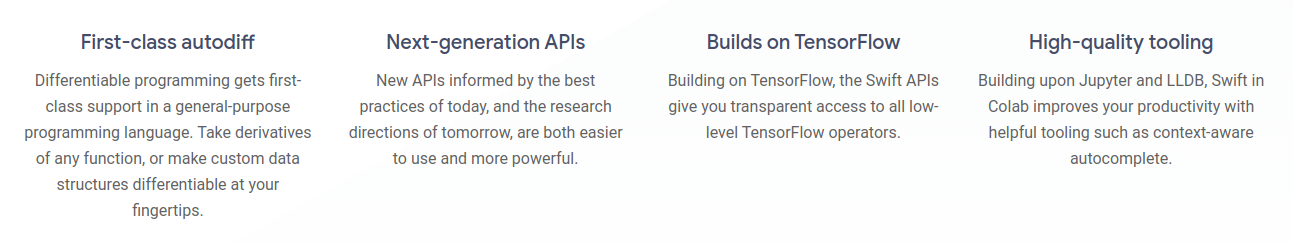
\includegraphics[width=\linewidth,keepaspectratio]{s4tf6}
\end{center}
\end{frame}

%%%%%%%%%%%%%%%%%%%%%%%%%%%%%%%%%%%%%%%%%%%%%%%%%%%
\begin{frame}[fragile] \frametitle{Swift for Tensorflow}

\begin{center}
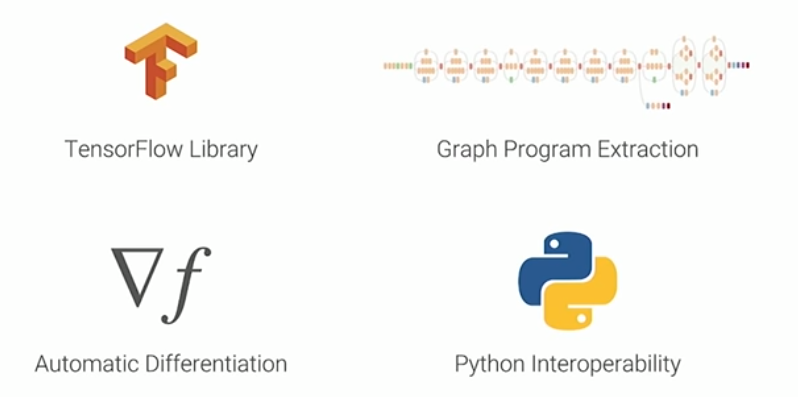
\includegraphics[width=\linewidth,keepaspectratio]{s4tf9}
\end{center}

{\tiny (Ref: Swift for TensorFlow (TensorFlow @ O’Reilly AI Conference, San Francisco '18) - Richard Wei)}
\end{frame}


%%%%%%%%%%%%%%%%%%%%%%%%%%%%%%%%%%%%%%%%%%%%%%%%%%%
\begin{frame}[fragile] \frametitle{Sample Neural Network}

\begin{center}
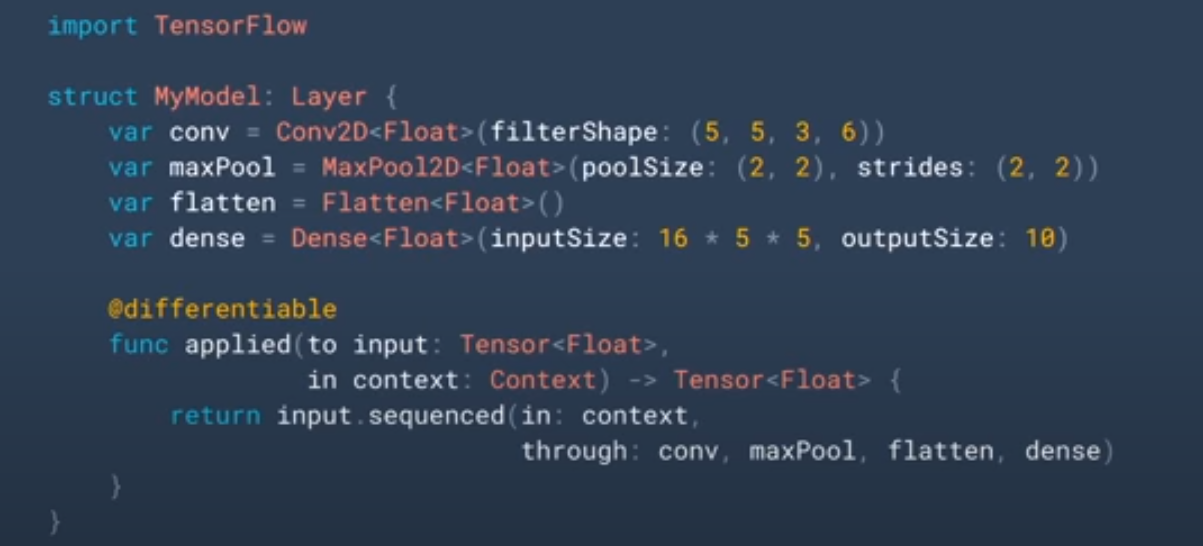
\includegraphics[width=0.65\linewidth,keepaspectratio]{s4tf7}

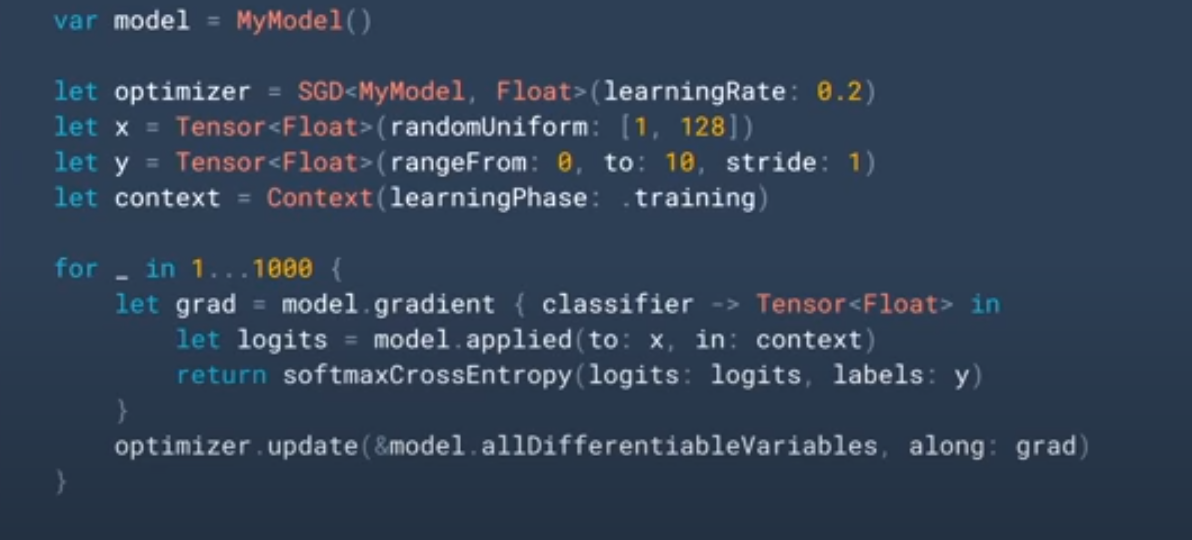
\includegraphics[width=0.65\linewidth,keepaspectratio]{s4tf8}
\end{center}

{\tiny (Ref: Swift for TensorFlow: The Next-Generation Machine Learning Framework (TF Dev Summit '19))}
\end{frame}

%%%%%%%%%%%%%%%%%%%%%%%%%%%%%%%%%%%%%%%%%%%%%%%%%%%
\begin{frame}[fragile] \frametitle{Graph Program Execution}

Why Swift For TensorFlow is fast even if its written like in Python like manner or like Eager execution way?

\begin{itemize}
\item Although it is creating graphs in the backend [like TensorFlow] but you don’t have to create sessions for executing these graphs, explicitly. Handled internally. Called ``Define-by-Run design'' ie no sessions required ie Eager like execution.
\item Ifs, Loops, MatMul, Zip, etc Ops are identified and directly compiled into TensorFlow graphs, the binaries.
\item As its compiling the graph, it catches errors (such as shape errors or type errors) as well, before running.
\end{itemize}

\begin{center}
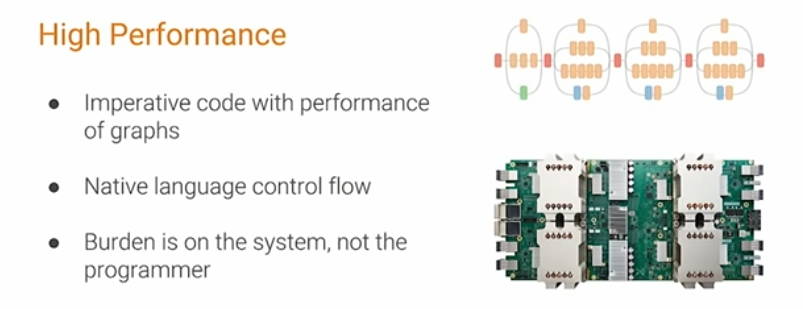
\includegraphics[width=0.5\linewidth,keepaspectratio]{s4tf10}
\end{center}
\end{frame}

%%%%%%%%%%%%%%%%%%%%%%%%%%%%%%%%%%%%%%%%%%%%%%%%%%%
\begin{frame}[fragile] \frametitle{Automatic Differentiation}

\begin{itemize}
\item AutoDiff (or AutoGrad in case of PyTorch) is generally implemented in library but for Swift its part of the language.
\item Works on standard library types, functions, etc. and also can make custom data structures, types differentiable as well.
\item Supports two differential functions: \lstinline|#gradient(of:withRespectTo:)| and \lstinline|#valueAndGradient(of:)|
\end{itemize}

\begin{center}
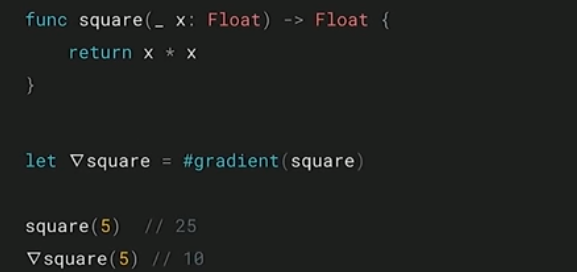
\includegraphics[width=0.5\linewidth,keepaspectratio]{s4tf11}
\end{center}
\end{frame}

%%%%%%%%%%%%%%%%%%%%%%%%%%%%%%%%%%%%%%%%%%%%%%%%%%%
\begin{frame}[fragile] \frametitle{Automatic Differentiation}

Syntax for \lstinline|#gradient|

\begin{center}
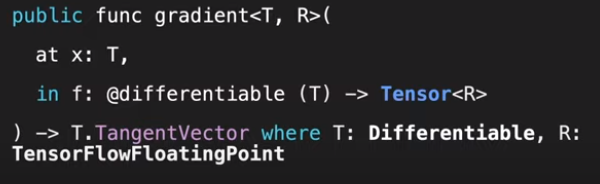
\includegraphics[width=0.5\linewidth,keepaspectratio]{s4tf13}
\end{center}


\begin{itemize}
\item Takes 'x' of generic type `T', 'at' needs to value at which derivative has to be computed, 'in' is either pre-writtent differentiable function or an inline closure code, with generic return type `R'. Returns derivative as \lstinline|T.TangentVector| where T (say, Float) is differentiable (btw, Int is not) and `R' is Float again (cant be Int).
\item Compiler catches errors pointing to non-differentiable op.
\item Currently only automatic reverse differentiation is allowed and forward differentiation is in discussions.
\end{itemize}


\end{frame}


%%%%%%%%%%%%%%%%%%%%%%%%%%%%%%%%%%%%%%%%%%%%%%%%%%%%%%%%%%%%%%%%%%%%%%%%%%%%%%%%%%
\begin{frame}[fragile]\frametitle{}
\begin{center}
{\Large Getting Started: Installation}
\end{center}
\end{frame}

%%%%%%%%%%%%%%%%%%%%%%%%%%%%%%%%%%%%%%%%%%%%%%%%%%%%%%%%%%%
\begin{frame} \frametitle{Best way to use Swift}

\begin{itemize}
\item Use Google Colab
\item Copy https://colab.research.google.com/github/tensorflow/ swift/blob/master/notebooks/blank\_swift.ipynb to your Google Drive
\item Rename it properly and start using \ldots
\item Or Open https://colab.research.google.com/notebook\#create =true\&language=swift and then save it to GDrive.
\item If you want to have it locally, then go ahead \ldots
\end{itemize}

\end{frame}


%%%%%%%%%%%%%%%%%%%%%%%%%%%%%%%%%%%%%%%%%%%%%%%%%%%%%%%%%%%
\begin{frame} \frametitle{Installation on Windows}
\begin{itemize}
\item NO NEED TO Download RELEASE toolchain and sig from https://swift.org/download/ but get it from "Development Snapshots" of Windows from https://github.com/tensorflow/swift/blob/master/Installation.md

\item \lstinline|gpg.exe --import all-keys.asc| from https://swift.org/keys/all-keys.asc
\item Install exe
\item It gets installed in \lstinline|C:\\Library\\Developer\\Toolchains|
\item Define SDKROOT in Env Variables (..shown in next slide)
\end{itemize}

{\tiny (Note:  The .exe installer for Windows are signed using GnuPG with one of the keys of the Swift open source project. Everyone is strongly encouraged to verify the signatures before using the software.). For Other OSs refer https://swift.org/getting-started/\#installing-swift}
\end{frame}

%%%%%%%%%%%%%%%%%%%%%%%%%%%%%%%%%%%%%%%%%%%%%%%%%%%%%%%%%%%
\begin{frame} \frametitle{Installation on Windows}
\begin{itemize}

\item From an (elevated) "Administrator" x64 Native Tools for VS2019 Command Prompt shell (Follow step 4 mentioned in link above)
\item Set \lstinline|SDKROOT=C:/Library/Developer/Platforms/| \lstinline|Windows.platform/Developer/SDKs/Windows.sdk|
\item Create test.swift with code as \lstinline|print("hello")| and run
\item \lstinline|swiftc -sdk \%SDKROOT\% -I \%SDKROOT\%/usr/lib/swift -L \%SDKROOT\%/usr/lib/swift/windows -emit-executable -o test.exe test.swift|
\item \lstinline|test.exe|
\end{itemize}
{\tiny (Note:  Interpreter mode and direct invocation from VS 2019 are currently not supported on Windows.. Ref: https://github.com/tensorflow/swift/blob/master/Installation.md)}
\end{frame}


%%%%%%%%%%%%%%%%%%%%%%%%%%%%%%%%%%%%%%%%%%%%%%%%%%%%%%%%%%%
\begin{frame} \frametitle{Jupyter Installation on Windows}

Assuming "Swift for Tensorflow" toolchain is already installed

\begin{itemize}
\item git clone https://github.com/google/swift-jupyter.git
\item cd swift-jupyter
\item conda create -n swift-tensorflow python==3.6
\item activate swift-tensorflow
\item conda install jupyter numpy matplotlib
\item python register.py --sys-prefix --swift-python-use-conda --use-conda-shared-libs --swift-toolchain path-to-unknown-Asserts-development.xctoolchain
\end{itemize}

{\tiny (Note:Error "ModuleNotFoundError: No module named '\_lldb'" (Track: https://github.com/google /swift-jupyter/issues/98)}
 
\end{frame}


%%%%%%%%%%%%%%%%%%%%%%%%%%%%%%%%%%%%%%%%%%%%%%%%%%%%%%%%%%%%%%%%%%%%%%%%%%%%%%%%%%
\begin{frame}[fragile]\frametitle{}
\begin{center}
{\Large Swift for Tensorflow Basic Neural Network: Step by Step}
\end{center}
\end{frame}

%%%%%%%%%%%%%%%%%%%%%%%%%%%%%%%%%%%%%%%%%%%%%%%%%%%%%%%%%%%
\begin{frame}[fragile] \frametitle{Model Building}

\begin{itemize}
\item Model is defined by confirming to \lstinline|Layer| protocol.
\item Within Model definition, you can add further layers.
\item \lstinline|Dense| itself is confirming to \lstinline|Layer| protocol and has Weights and Biases stored.
\end{itemize}

\begin{center}
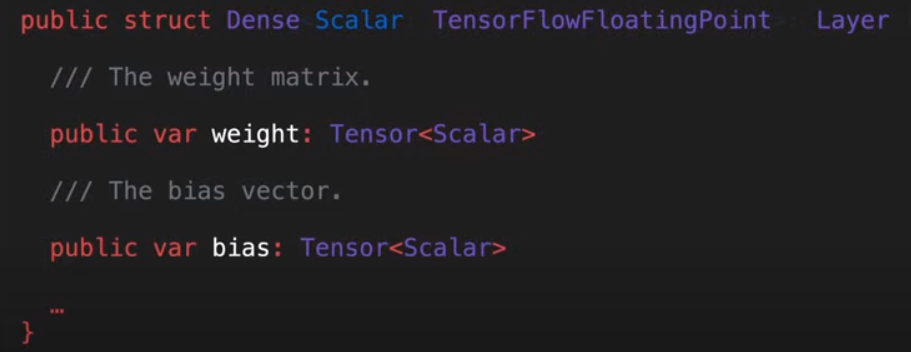
\includegraphics[width=0.8\linewidth,keepaspectratio]{s4tf14}
\end{center}


{\tiny (Ref:Introduction to Swift for TensorFlow by Devesh Shetty)}

\end{frame}

%%%%%%%%%%%%%%%%%%%%%%%%%%%%%%%%%%%%%%%%%%%%%%%%%%%%%%%%%%%
\begin{frame}[fragile] \frametitle{Model Building}

As part of confirmation to \lstinline|Layer| protocol we need to make this \lstinline|struct| callable as a function.

\begin{lstlisting}
model = MagicalModel()
model(input) # Thats calling model as a function.
\end{lstlisting}


\begin{center}
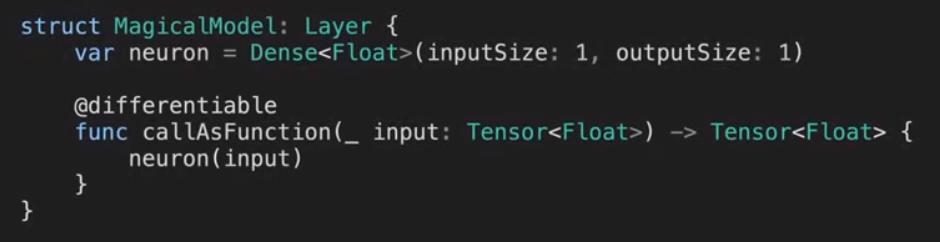
\includegraphics[width=\linewidth,keepaspectratio]{s4tf15}
\end{center}


{\tiny (Ref:Introduction to Swift for TensorFlow by Devesh Shetty)}

\end{frame}



%%%%%%%%%%%%%%%%%%%%%%%%%%%%%%%%%%%%%%%%%%%%%%%%%%%%%%%%%%%
\begin{frame}[fragile] \frametitle{Define a model}

\begin{lstlisting}[basicstyle=\scriptsize]
import TensorFlow
let hiddenSize: Int = 10
struct Model: Layer {
    var layer1 = Dense<Float>(inputSize: 4, outputSize: hiddenSize, activation: relu)
    var layer2 = Dense<Float>(inputSize: hiddenSize, outputSize: hiddenSize, activation: relu)
    var layer3 = Dense<Float>(inputSize: hiddenSize, outputSize: 3, activation: identity)
    
    @differentiable
    func callAsFunction(_ input: Tensor<Float>) -> Tensor<Float> {
        return input.sequenced(through: layer1, layer2, layer3)
    }
}
\end{lstlisting}

\lstinline|Layer| is a protocol thats being adopted for Model


\end{frame}

%%%%%%%%%%%%%%%%%%%%%%%%%%%%%%%%%%%%%%%%%%%%%%%%%%%%%%%%%%%
\begin{frame}[fragile] \frametitle{Model Compilation and Data}


\begin{lstlisting}[basicstyle=\scriptsize]
var classifier = Model()
let optimizer = SGD(for: classifier, learningRate: 0.02)
Context.local.learningPhase = .training

// Dummy data.
let x: Tensor<Float> = Tensor(randomNormal: [100, 4])
let y: Tensor<Int32> = Tensor(randomUniform: [100])
\end{lstlisting}

\lstinline|learningPhase| is an enum predefined with values as:


\begin{center}
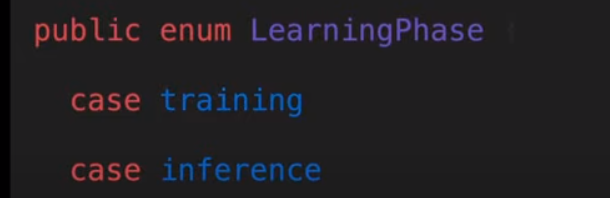
\includegraphics[width=0.6\linewidth,keepaspectratio]{s4tf16}
\end{center}



\end{frame}

%%%%%%%%%%%%%%%%%%%%%%%%%%%%%%%%%%%%%%%%%%%%%%%%%%%%%%%%%%%
\begin{frame}[fragile] \frametitle{Optimizer}

\begin{itemize}
\item  \lstinline|optimizr.update| is defined as mutating.
\item The model is passed with an \lstinline|&| meaning its reference-pointer variable, used as \lstinline|inout|, meaning both, `in' and `out'.
\end{itemize}

\begin{center}
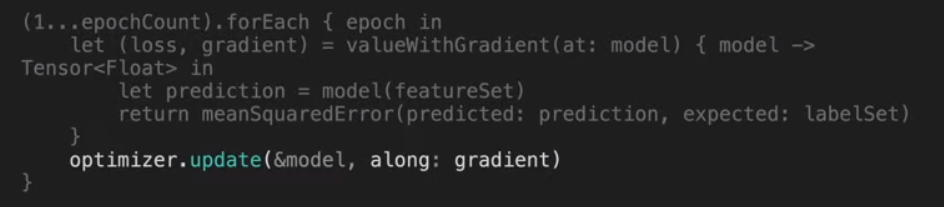
\includegraphics[width=\linewidth,keepaspectratio]{s4tf17}
\end{center}


{\tiny (Ref:Introduction to Swift for TensorFlow by Devesh Shetty)}

\end{frame}

%%%%%%%%%%%%%%%%%%%%%%%%%%%%%%%%%%%%%%%%%%%%%%%%%%%%%%%%%%%
\begin{frame}[fragile] \frametitle{Model Training}

\begin{center}
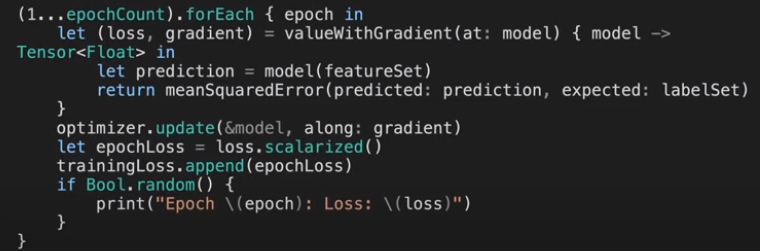
\includegraphics[width=\linewidth,keepaspectratio]{s4tf18}
\end{center}


{\tiny (Ref:Introduction to Swift for TensorFlow by Devesh Shetty)}

\end{frame}

%%%%%%%%%%%%%%%%%%%%%%%%%%%%%%%%%%%%%%%%%%%%%%%%%%%%%%%%%%%
\begin{frame}[fragile] \frametitle{Model Training}

One way to define a training epoch is to use the \lstinline|gradient(at:in:)| function. Inside \lstinline|gradient| you can specify differentiable function name or write a Closure code directly.

\begin{lstlisting}[basicstyle=\scriptsize]
for _ in 0..<1000 {
    let grad_model = gradient(at: classifier) { classifier -> Tensor<Float> in
        let y_pred = classifier(x)
        let loss = softmaxCrossEntropy(logits: y_pred, labels: y)
        print("Loss: \(loss)")
        return loss
    }
    optimizer.update(&classifier, along: grad_model)
}
\end{lstlisting}

% \begin{center}
% 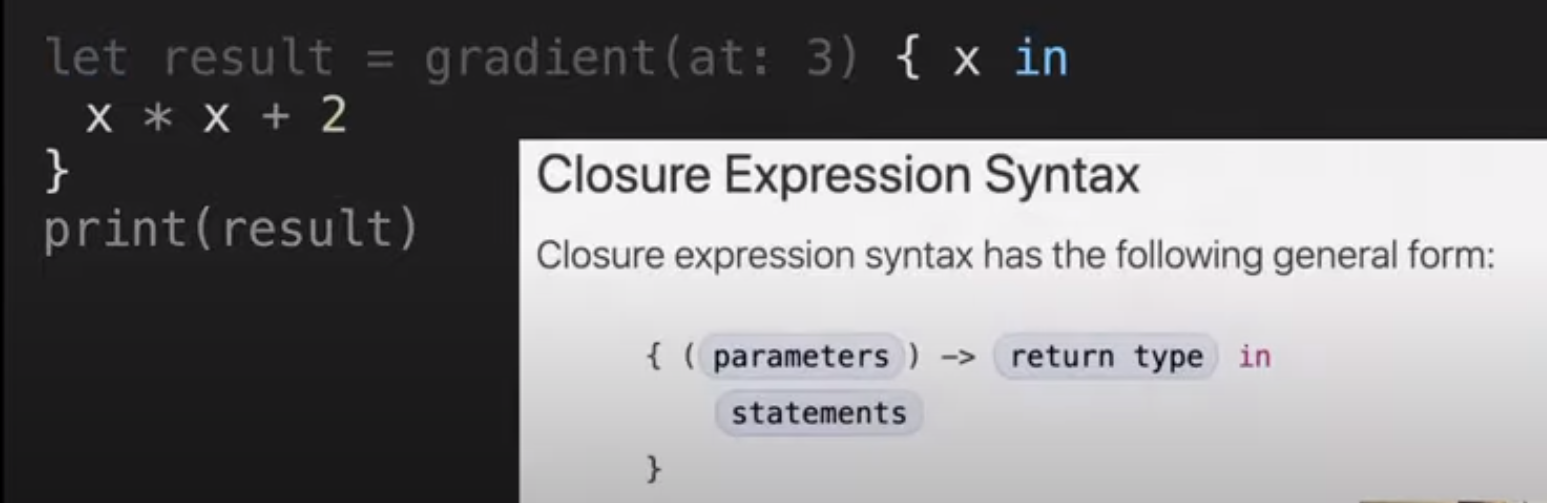
\includegraphics[width=0.6\linewidth,keepaspectratio]{s4tf12}
% \end{center}


Another way \ldots [PTO]

\end{frame}

%%%%%%%%%%%%%%%%%%%%%%%%%%%%%%%%%%%%%%%%%%%%%%%%%%%%%%%%%%%
\begin{frame}[fragile] \frametitle{Model Training}

Make use of methods on \lstinline|Differentiable| or \lstinline|Layer| that produce a backpropagation function. This allows you to compose your derivative computation with great flexibility.

\begin{lstlisting}[basicstyle=\scriptsize]
for _ in 0..<1000 {
    let (y_pred, backprop) = classifier.appliedForBackpropagation(to: x)
    let (loss, grad_y_pred) = valueWithGradient(at: y_pred) { y_pred in softmaxCrossEntropy(logits: y_pred, labels: y) }
    print("Model output: \(y_pred), Loss: \(loss)")
    let (grad_model, _) = backprop(grad_y_pred)
    optimizer.update(&classifier, along: grad_model)
\end{lstlisting}

\end{frame}

%%%%%%%%%%%%%%%%%%%%%%%%%%%%%%%%%%%%%%%%%%%%%%%%%%%%%%%%%%%
\begin{frame}[fragile] \frametitle{Inferencing}

\begin{center}
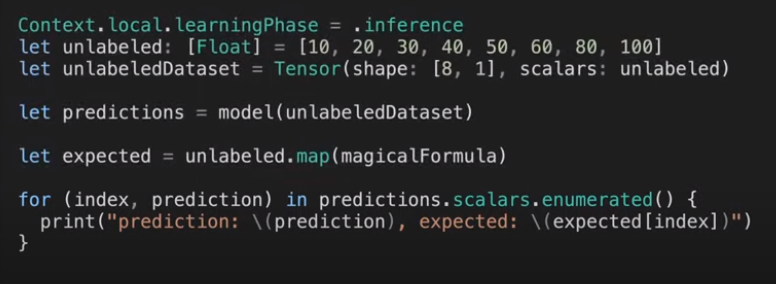
\includegraphics[width=\linewidth,keepaspectratio]{s4tf19}

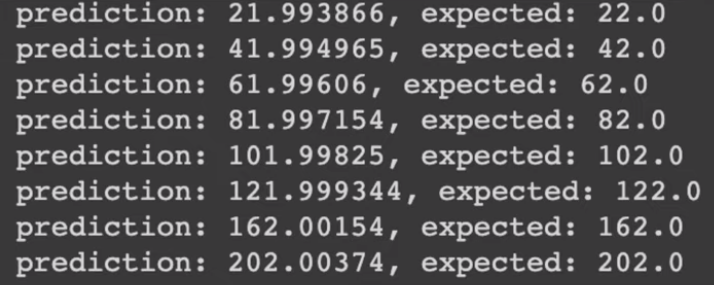
\includegraphics[width=0.6\linewidth,keepaspectratio]{s4tf20}

\end{center}


{\tiny (Ref:Introduction to Swift for TensorFlow by Devesh Shetty)}

\end{frame}

%%%%%%%%%%%%%%%%%%%%%%%%%%%%%%%%%%%%%%%%%%%%%%%%%%%%%%%%%%%%%%%%%%%%%%%%%%%%%%%%%%
\begin{frame}[fragile]\frametitle{}
\begin{center}
{\Large MNIST: Step by Step}

{\tiny (Ref: https://github.com/tensorflow/swift-models/tree/master/Examples/LeNet-MNIST)}

\end{center}
\end{frame}

%%%%%%%%%%%%%%%%%%%%%%%%%%%%%%%%%%%%%%%%%%%%%%%%%%%%%%%%%%%
\begin{frame}[fragile] \frametitle{Prerequisite Installations}

\begin{itemize}
\item Need \lstinline|ImageClassificationModels| and \lstinline|Datasets|
\item Since swift-models is set up as a Swift package, we call the repo as a package and provide the URL and branch we want to use (you can also set to version, instead)
\item As both from same repo/package, no 2 separate lines
\end{itemize}

\begin{lstlisting}[basicstyle=\scriptsize]
%install `.package(url: ``https://github.com/tensorflow/swift-models.git'', .branch(``master''))' ImageClassificationModels Datasets

import TensorFlow
import Datasets
import ImageClassificationModels
\end{lstlisting}


\end{frame}

% %%%%%%%%%%%%%%%%%%%%%%%%%%%%%%%%%%%%%%%%%%%%%%%%%%%%%%%%%%%
% \begin{frame}[fragile] \frametitle{Data Loading}

% \begin{center}
% 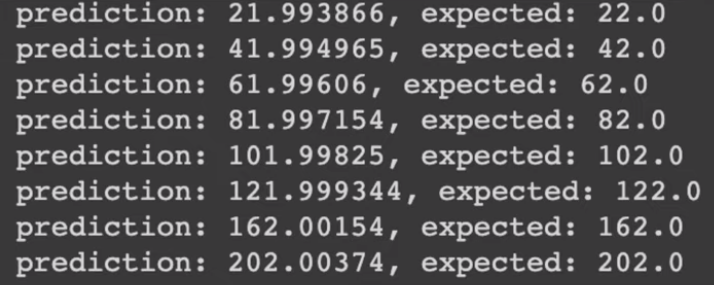
\includegraphics[width=\linewidth,keepaspectratio]{s4tf20}
% \end{center}


% {\tiny (Ref:Introduction to Swift for TensorFlow by Devesh Shetty)}

% \end{frame}


%%%%%%%%%%%%%%%%%%%%%%%%%%%%%%%%%%%%%%%%%%%%%%%%%%%%%%%%%%%
\begin{frame}[fragile] \frametitle{Model}

\begin{itemize}
\item Model is built as a Swift \lstinline|struct| that extends the \lstinline|Layer| protocol, which represents a neural network layer. 
\item The protocol expects to take an input, pass it through the layer, and return the resulting output. 
\item This is enforced by having the \lstinline|struct| conform to \lstinline|callAsFunction|
\end{itemize}


\begin{lstlisting}[basicstyle=\scriptsize]
@differentiable
public func callAsFunction(_ input: Tensor<Float>) -> Tensor<Float> { 
  let convolved = input.sequenced(through: conv1, pool1, conv2, pool2) 
  return convolved.sequenced(through: flatten, fc1, fc2, fc3) 
}
\end{lstlisting}

{\tiny (Ref: https://github.com/tensorflow/swift-models/blob/master/Models/ImageClassification/LeNet-5.swift )}

\end{frame}

%%%%%%%%%%%%%%%%%%%%%%%%%%%%%%%%%%%%%%%%%%%%%%%%%%%%%%%%%%%
\begin{frame}[fragile] \frametitle{LeNet}

\begin{lstlisting}[basicstyle=\scriptsize]
public struct LeNet: Layer {
   public var conv1 = Conv2D<Float>(filterShape: (5, 5, 1, 6), padding: .same, activation: relu)
   public var pool1 = AvgPool2D<Float>(poolSize: (2, 2), strides: (2, 2))
   public var conv2 = Conv2D<Float>(filterShape: (5, 5, 6, 16), activation: relu)
   public var pool2 = AvgPool2D<Float>(poolSize: (2, 2), strides: (2, 2))
   public var flatten = Flatten<Float>()
   public var fc1 = Dense<Float>(inputSize: 400, outputSize: 120, activation: relu)
   public var fc2 = Dense<Float>(inputSize: 120, outputSize: 84, activation: relu)
   public var fc3 = Dense<Float>(inputSize: 84, outputSize: 10, activation: softmax)
  public init() {}
}
\end{lstlisting}

{\tiny (Ref: https://github.com/tensorflow/swift-models/blob/master/Models/ImageClassification/LeNet-5.swift )}

\end{frame}

%%%%%%%%%%%%%%%%%%%%%%%%%%%%%%%%%%%%%%%%%%%%%%%%%%%%%%%%%%%
\begin{frame}[fragile] \frametitle{Benchmarking with Stats}

Collect accuracy values while training and testing in a \lstinline|struct|.

\begin{lstlisting}[basicstyle=\scriptsize]
struct Statistics {
  var correctGuessCount: Int = 0
  var totalGuessCount: Int = 0
  var totalLoss: Float =
  mutating func updateGuessCounts(logits: Tensor<Float>, labels: Tensor<Int32>, batchSize: Int) {
    let correctPredictions = logits.argmax(squeezingAxis: 1) .== labels
    self.correctGuessCount += Int(
   Tensor<Int32>(correctPredictions).sum().scalarized())
   self.totalGuessCount += batchSize
  }
}
\end{lstlisting}

\end{frame}

%%%%%%%%%%%%%%%%%%%%%%%%%%%%%%%%%%%%%%%%%%%%%%%%%%%%%%%%%%%
\begin{frame}[fragile] \frametitle{Training}

\begin{lstlisting}[basicstyle=\scriptsize]
// The training loop.
for epoch in 1...epochCount {
    var trainStats = Statistics()
    var testStats = Statistics()
    Context.local.learningPhase = .training
    for i in 0 ..< dataset.trainingSize / batchSize {
        let images = dataset.trainingImages.minibatch(at: i, batchSize: batchSize)
        let labels = dataset.trainingLabels.minibatch(at: i, batchSize: batchSize)
        // Compute the gradient with respect to the model.
        let (loss, gradients) = valueWithGradient(at: model) { model -> Tensor<Float> in
            let logits = model(images)
            trainStats.updateGuessCounts(logits: logits, labels: labels, batchSize: batchSize)
            return softmaxCrossEntropy(logits: logits, labels: labels)
        }
        trainStats.totalLoss += loss.scalarized()
        optimizer.update(&model, along: gradients)
    }
\end{lstlisting}

\end{frame}

%%%%%%%%%%%%%%%%%%%%%%%%%%%%%%%%%%%%%%%%%%%%%%%%%%%%%%%%%%%
\begin{frame}[fragile] \frametitle{Testing}

\begin{lstlisting}[basicstyle=\scriptsize]
// The training loop.
for epoch in 1...epochCount {
			// Training loop
			Context.local.learningPhase = .inference
			for i in 0 ..< dataset.testSize / batchSize {
					let images = dataset.testImages.minibatch(at: i, batchSize: batchSize)
					let labels = dataset.testLabels.minibatch(at: i, batchSize: batchSize)
					// Compute loss on test set
					let logits = model(images)
					testStats.updateGuessCounts(logits: logits, labels: labels, batchSize: batchSize)
					let loss = softmaxCrossEntropy(logits: logits, labels: labels)
					testStats.totalLoss += loss.scalarized()
			}			
    }
\end{lstlisting}

\end{frame}

%%%%%%%%%%%%%%%%%%%%%%%%%%%%%%%%%%%%%%%%%%%%%%%%%%%%%%%%%%%
\begin{frame}[fragile] \frametitle{Logging}

\begin{lstlisting}[basicstyle=\scriptsize]
// The training loop.
for epoch in 1...epochCount {
			// Training loop
			// Testing loop
			let trainAccuracy = Float(trainStats.correctGuessCount) / Float(trainStats.totalGuessCount)
			let testAccuracy = Float(testStats.correctGuessCount) / Float(testStats.totalGuessCount)
			print("""
						[Epoch \(epoch)] \
						Training Loss: \(trainStats.totalLoss), \
						Training Accuracy: \(trainStats.correctGuessCount)/\(trainStats.totalGuessCount) \
						(\(trainAccuracy)), \
						Test Loss: \(testStats.totalLoss), \
						Test Accuracy: \(testStats.correctGuessCount)/\(testStats.totalGuessCount) \
						(\(testAccuracy))
						""")			
    }
\end{lstlisting}

\end{frame}

%%%%%%%%%%%%%%%%%%%%%%%%%%%%%%%%%%%%%%%%%%%%%%%%%%%%%%%%%%%
\begin{frame}[fragile] \frametitle{Results}

\begin{lstlisting}[basicstyle=\scriptsize]
Beginning training ...
[Epoch 1] Training Loss: 957.23724, Training Accuracy: 27154/59904 (0.45329192), Test Loss: 128.8437, Test Accuracy: 8156/9984 (0.81690705) 
[Epoch 2] Training Loss: 768.2697, Training Accuracy: 49305/59904 (0.8230669), Test Loss: 126.20526, Test Accuracy: 8441/9984 (0.8454527) 
...
[Epoch 12] Training Loss: 695.9648, Training Accuracy: 58446/59904 (0.97566104), Test Loss: 116.18148, Test Accuracy: 9723/9984 (0.9738582)
\end{lstlisting}

Good accuracy!!

\end{frame}

%%%%%%%%%%%%%%%%%%%%%%%%%%%%%%%%%%%%%%%%%%%%%%%%%%%%%%%%%%%%%%%%%%%%%%%%%%%%%%%%%%
\begin{frame}[fragile]\frametitle{}
\begin{center}
{\Large What Next \ldots }
\end{center}
\end{frame}

%%%%%%%%%%%%%%%%%%%%%%%%%%%%%%%%%%%%%%%%%%%%%%%%%%%
\begin{frame}[fragile] \frametitle{Practice}

\begin{itemize}
\item The iris classification problem https://www.tensorflow.org/swift/tutorials/model \_training\_walkthrough
\end{itemize}

\end{frame}


%%%%%%%%%%%%%%%%%%%%%%%%%%%%%%%%%%%%%%%%%%%%%%%%%%%
\begin{frame}[fragile] \frametitle{Future of Swift for Tensorflow}

\begin{itemize}
\item Currently, it is in infancy and the libraries around data science and numeric computing are still developing.
\item Has a strong industry backing behind it.
\item Swift will have a rich ecosystem of tools and libraries- maybe even better than what Python has today.
\end{itemize}

\end{frame}
